\documentclass{article}
\usepackage{graphicx}
\usepackage{amsmath}
\usepackage{amssymb}
\usepackage{float}
\usepackage{tikz}
\usetikzlibrary{positioning, arrows.meta}

\title{Signal Processing: An Introduction}
\author{Badger Code}
\date{\today}

\begin{document}
\maketitle

\section{Introduction}
Signal processing is a fundamental discipline in various fields, including telecommunications, audio processing, image processing, and more. It involves the analysis, manipulation, and interpretation of signals to extract relevant information or improve signal quality. A signal can be any time-varying phenomenon that carries information. Examples include audio waveforms, electromagnetic signals, and image pixel intensities.

This paper aims to provide a comprehensive overview of signal processing techniques, including basic concepts, mathematical tools, and practical examples. We will explore different types of signals, discuss common signal processing operations, and present various methods for signal analysis and enhancement.

In this section, we will briefly discuss the concept of signals and their representation in the time and frequency domains. Additionally, we will introduce the Fourier Transform, which is a fundamental tool in signal processing.

\subsection{Time-Domain Representation}
A signal can be represented in the time domain as a function $x(t)$, where $t$ represents time. The amplitude of the signal varies with time, and it can be continuous or discrete. A continuous-time signal can be represented as a function $x(t)$, whereas a discrete-time signal is represented as a sequence $\{x[n]\}$.

\subsection{Frequency-Domain Representation}
The frequency-domain representation of a signal provides insights into the frequency content of the signal. The Fourier Transform is a valuable mathematical tool used to convert a signal from the time domain to the frequency domain. It decomposes the signal into its constituent frequencies, revealing the amplitude and phase of each frequency component.

The continuous Fourier Transform of a continuous-time signal $x(t)$ is defined as follows:

\begin{equation}
X(f) = \int_{-\infty}^{\infty} x(t) \cdot e^{-j2\pi ft} \, dt
\end{equation}

Where:
$X(f)$ - The complex-valued representation of the signal in the frequency domain.
$j$ - The imaginary unit.
$f$ - The frequency variable in Hertz (Hz).

Similarly, the discrete Fourier Transform (DFT) of a discrete-time signal $\{x[n]\}$ is given by:

\begin{equation}
X[k] = \sum_{n=0}^{N-1} x[n] \cdot e^{-j2\pi kn/N}
\end{equation}

Where:
$X[k]$ - The complex-valued representation of the signal in the frequency domain.
$N$ - The number of samples in the signal.
$k$ - The frequency index, ranging from 0 to $N-1$.

The inverse Fourier Transform allows us to reconstruct the original signal from its frequency-domain representation:

\begin{equation}
x(t) = \int_{-\infty}^{\infty} X(f) \cdot e^{j2\pi ft} \, df
\end{equation}

Or for the discrete case:

\begin{equation}
x[n] = \frac{1}{N} \sum_{k=0}^{N-1} X[k] \cdot e^{j2\pi kn/N}
\end{equation}

The Fourier Transform is a powerful tool that enables us to analyze the frequency components of a signal and perform various operations in the frequency domain, such as filtering and modulation. Next, we will demonstrate some basic signal processing operations using the Fourier Transform.

\section{Basic Signal Processing Operations}
In this section, we will explore some fundamental signal processing operations, including signal filtering and signal modulation. We will use the Fourier Transform to illustrate these concepts.

\subsection{Signal Filtering}
Signal filtering is a common signal processing operation used to remove or attenuate unwanted frequency components from a signal while preserving the desired components. The frequency response of a filter determines how it affects different frequencies in the signal.

\subsection{Signal Filtering (continued)}
There are two primary types of filters: low-pass filters and high-pass filters. A low-pass filter allows low-frequency components to pass through while attenuating higher frequencies. Conversely, a high-pass filter attenuates low frequencies and allows higher frequencies to pass through.

The frequency response of a filter is often represented by its magnitude response $|H(f)|$, where $H(f)$ is the filter's frequency response in the complex plane. The phase response of the filter is denoted as $\angle H(f)$.

One common type of filter is the ideal low-pass filter, which has a rectangular frequency response. Let's consider an ideal low-pass filter with a cutoff frequency $f_c$. The frequency response $H(f)$ of this filter is given by:

\begin{equation}
H(f) = \begin{cases}
    1, & \text{if } |f| \leq f_c \\
    0, & \text{otherwise}
\end{cases}
\end{equation}

Let's visualize the frequency response of this ideal low-pass filter using a graph:

\begin{figure}[H]
    \centering
    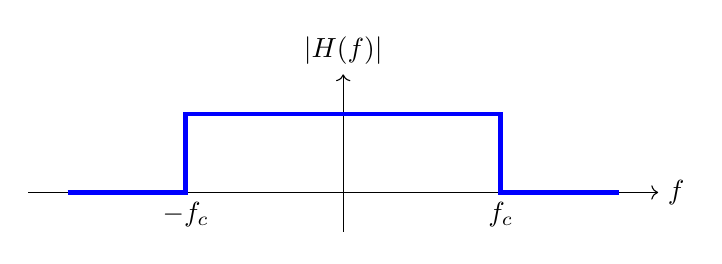
\begin{tikzpicture}
        \draw[->] (-4, 0) -- (4, 0) node[right] {$f$};
        \draw[->] (0, -0.5) -- (0, 1.5) node[above] {$|H(f)|$};
        \draw[-, ultra thick, blue] (-3.5, 0) -- (-2, 0) -- (-2, 1) -- (2, 1) -- (2, 0) -- (3.5, 0);
        \node[below] at (-2, 0) {$-f_c$};
        \node[below] at (2, 0) {$f_c$};
    \end{tikzpicture}
    \caption{Frequency Response of an Ideal Low-Pass Filter}
\end{figure}

In practice, it is not possible to implement an ideal filter, but various filter design techniques aim to approximate ideal characteristics.

\subsection{Signal Modulation}
Signal modulation is a process of superimposing a baseband signal onto a carrier signal. It is widely used in communication systems for transmission and reception of signals over long distances. One common modulation technique is amplitude modulation (AM).

Consider a baseband signal $x(t)$ with amplitude $A_m$ and a carrier signal $c(t)$ with amplitude $A_c$ and frequency $f_c$. The amplitude-modulated signal $y(t)$ is given by:

\begin{equation}
y(t) = (A_c + A_m \cdot x(t)) \cdot \cos(2\pi f_c t)
\end{equation}

Let's visualize the process of amplitude modulation by plotting the baseband signal, carrier signal, and the amplitude-modulated signal:

\begin{figure}[H]
    \centering
    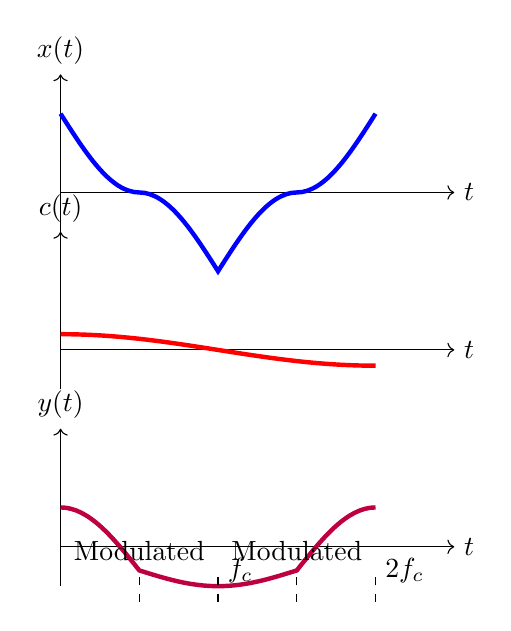
\begin{tikzpicture}
        % Baseband signal
        \draw[->] (0, -1.5) -- (0, 1.5) node[above] {$x(t)$};
        \draw[->] (0, 0) -- (5, 0) node[right] {$t$};
        \draw[-, ultra thick, blue] (0, 1) sin (1, 0) cos (2, -1) sin (3, 0) cos (4, 1);

        % Carrier signal
        \draw[->] (0, -2.5) -- (0, -0.5) node[above] {$c(t)$};
        \draw[->] (0, -2) -- (5, -2) node[right] {$t$};
        \draw[-, ultra thick, red] (0, -1.8) cos (2, -2) sin (4, -2.2);

        % Amplitude-modulated signal
        \draw[->] (0, -5) -- (0, -3) node[above] {$y(t)$};
        \draw[->] (0, -4.5) -- (5, -4.5) node[right] {$t$};
        \draw[-, ultra thick, purple] (0, -4) cos (1, -4.8) sin (2, -5) cos (3, -4.8) sin (4, -4);
        \draw[dashed] (2, -5.2) -- (2, -4.8) node[right] {$f_c$};
        \draw[dashed] (4, -5.2) -- (4, -4.8) node[right] {$2f_c$};
        \draw[dashed] (1, -5.2) -- (1, -4.8) node[above] {Modulated};
        \draw[dashed] (3, -5.2) -- (3, -4.8) node[above] {Modulated};
    \end{tikzpicture}
    \caption{Amplitude Modulation of a Baseband Signal with a Carrier Signal}
\end{figure}

As shown in the figure, the amplitude-modulated signal $y(t)$ contains the carrier frequency $f_c$ and two sidebands at frequencies $f_c + f_m$ and $f_c - f_m$, where $f_m$ is the frequency of the baseband signal. The modulated signal can be demodulated at the receiver to retrieve the original baseband signal.

\subsection{Conclusion}
In this paper, we provided an introduction to signal processing, covering key concepts such as time-domain and frequency-domain representations of signals. The Fourier Transform was introduced as a crucial tool for signal analysis in the frequency domain.

We explored basic signal processing operations, such as signal filtering, which is essential for removing unwanted noise and enhancing desired signals. We also discussed signal modulation, a technique widely used in communication systems to transmit signals efficiently.

Signal processing is a vast and exciting field with numerous applications in various domains. This paper serves as a foundation for further exploration of advanced signal processing techniques and their applications.

\end{document}